%%%%%%%%%%%%%%%%%%%%%%%%%% ch4
\begin{frame}
  \frametitle{主要内容}
  \tableofcontents[hideallsubsections]
\end{frame}

\section{随机过程的统计平均量(from ch2)}

\begin{frame}
\begin{block}{随机过程的均值$\mu_x(t)$: 表示随机过程在$t$时刻状态取值的理论平均值}
	\[\mu_x(t)\mathop{=}^{def}E[x(t)]=\int_{-\infty}^{\infty}xp(x;t)dx \]
	如果$x(t)$是电压或电流,则$\mu_x(t)$可以理解为在$t$时刻的``直流分量''。
\end{block}

\begin{block}{随机过程的均方值$\varphi_x^2(t)$}
	\[\varphi_x^2(t)\mathop{=}^{def}E[x^2(t)]=\int_{-\infty}^{\infty}x^2p(x;t)dx \]
	如果$x(t)$是电压或电流,则$\varphi_x^2(t)$可以理解在$t$时刻它在$1\Omega$电阻上消耗的``平均功率''。
\end{block}
\end{frame}

\begin{frame}
\begin{block}{随机过程的方差/标准偏差$\delta_x^2(t)$}
	\[\sigma_x^2(t)\mathop{=}^{def}E[(x(t)-\mu_x(t))^2]=\int_{-\infty}^{\infty}(x-\mu_x(t))^2p(x;t)dx \]
	方差$\sigma_x^2(t)$表示随机过程在$t$时刻取其值偏离其均值$\mu_x(t)$的离散程度。如果$x(t)$是电压或电流,则$\delta_x^2(t)$可以理解在$t$时刻它在$1\Omega$电阻上消耗的``交流功率''。
\end{block}
\begin{block}{均值$\mu_x(t)$,均方值$\varphi_x^2(t)$,方差$\delta_x^2(t)$之间的关系}
	\[\sigma_x^2(t)=\varphi_x^2(t)-\mu_x^2(t)\]
\end{block}
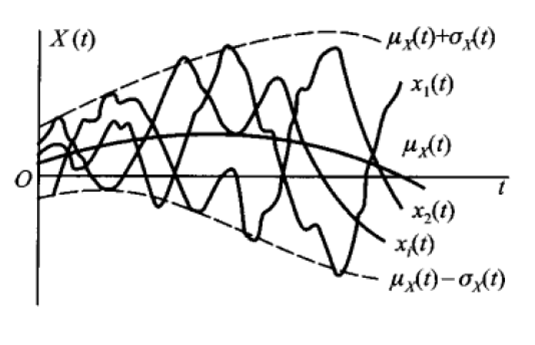
\includegraphics[scale=0.4]{delta}
\end{frame}

\begin{frame}
\begin{block}{随机过程的自相关函数$r_x(t_j,t_k)$}
	\begin{align*}
	r_x(t_j,t_k)&\mathop{=}^{def}E[x(t_j)x(t_k)]\\
	&=\int_{-\infty}^{\infty}	\int_{-\infty}^{\infty}x_jx_kp(x_j,x_k;t_j,t_k)dx_jdx_k
	\end{align*}
\end{block}
随机过程的自相关函数$r_x(t_j,t_k)$可以理解为它的两个随机变量$x(t_j)$与$x(t_k)$之间含有均值时的相关程度的度量。显然
\[r_x(t,t)=\varphi_x^2(t)\]
\end{frame}

\begin{frame}
\begin{block}{随机过程的自协方差函数$c_x(t_j,t_k)$}
	\begin{align*}
	c_x(t_j,t_k)&\mathop{=}^{def}E[((x(t_j)-\mu_x(t_j)(x(t_k)-\mu_x(t_k)]\\
	&=\int_{-\infty}^{\infty}\int_{-\infty}^{\infty}(x_j-\mu_x(t_j))(x_k-\mu_x(t_k))p(x_j,x_k;t_j,t_k)dx_idx_k
	\end{align*}
\end{block}
	随机过程的自协方差函数$c_x(t_j,t_k)$可以理解为它的两个随机变量$x(t_j)$与$x(t_k)$之间的相关程度的度量。它们的自相关系数定义为
\[\rho_x(t_j,t_k)\mathop{=}^{def}\frac{c_x(t_j,t_k)}{\sigma_x(t_j)\sigma_x(t_k)}\]
易证
\[c_x(t_j,t_k)=r_x(t_j,t_k)-\mu_x(t_j)\mu_x(t_k)\]
\[c_x(t,t)=\sigma_x^2(t)\]
\end{frame}

\begin{frame}
\begin{block}{随机过程的互相关函数$r_{xy}(t_j,t_k)$}
	\begin{align*}
	r_{xy}(t_j,t_k) &\mathop{=}^{def}E[x(t_j)y(t_k)]\\
	&=\int_{-\infty}^{\infty}\int_{-\infty}^{\infty}x_jy_kp(x_j,t_j;y_k,t_k)dx_jdy_k
	\end{align*}
	式中, $p(x_j,t_j;y_k,t_k)$是$x(t)$与$y(t)$的二维混合概率密度函数。
\end{block}
\end{frame}

\begin{frame}
\begin{block}{随机过程的互协方差函数$c_{xy}(t_j,t_k)$}
\begin{align*}
c_{xy}(t_j,t_k)&\mathop{=}^{def}E[(x(t_j)-\mu_x(t_j))(y(t_k)-\mu_x(t_k))]\\
&=\int_{-\infty}^{\infty}\int_{-\infty}^{\infty}(x_j-\mu_x(t_j))(y_k-\mu_x(t_k))p(x_j,t_j;x_k,t_k)dx_jdy_k
\end{align*}
\end{block}
随机过程$x(t)$和$y(t)$的互协方差函数$c_{xy}(t_j,t_k)$可以理解为它们各自的随机变量$x(t_j)$与$y(t_k)$之间的相关程度, 实际上表示两个随机过程$x(t)$与$y(t)$之间的相关程度。它们的互相关系数定义为
\[\rho_{xy}(t_j,t_k)\mathop{=}^{def}\frac{c_{xy}(t_j,t_k)}{\sigma_x(t_j)\sigma_x(t_k)}\]
易证
\[c_{xy}(t_j,t_k)=r_{xy}(t_j,t_k)-\mu_x(t_j)\mu_y(t_k)\]
\end{frame}

\section{随机过程的平稳性}

\begin{frame}
\begin{definition}[广义平稳随机过程,简称平稳随机过程]
	随机过程$x(t)$的平均统计量满足
	\begin{enumerate}
		\item $x(t)$的均值是与时间$t$无关的常数,即
		\[E[x(t)]=\mu_x\]
		\item $x(t)$的自相关函数只取决于时间间隔$\tau=t_k-t_j$,而与时间的起始时刻无关,即
		\[E[x(t_j)x(t_k)]=E[x(t_j)x(t_j+\tau)]=r_x(\tau) \]
	\end{enumerate}
\end{definition}
\end{frame}

\begin{frame}{平稳随机过程的统计平均量之间的关系}
平稳随机过程x(t)的均值$\mu_x$, 均方值$\varphi_x^2$, 方差$\sigma_x^2$,自相关函数$r_x(\tau)$,自协方差函数$c_x(\tau)$之间的关系
\begin{align*}
&\sigma_x^2=\varphi_x^2-\mu_x^2\\
&r_x(\tau)=r_x(-\tau)\\
&c_x(\tau)=r_x(\tau)-\mu_x^2\\
&c_x(\tau)=c_x(-\tau)\\
&\varphi_x^2=r_x(0)\\
&\sigma_x^2=c_x(0)\\
&r_x(0)\ge|r_x(\tau)|, \tau\ne 0\\
&c_x(0)\ge|c_x(\tau)|, \tau\ne 0
\end{align*}
\end{frame}

\begin{frame}
\begin{definition}[联合平稳随机过程]
	设$x(t)$和$y(t)$分别是两个平稳的随机过程, 如果对于任意的$\Delta t$, 有$r_{xy}(t_j+\Delta t,t_k+\Delta t)=r_{xy}(t_j,t_k)$, 即互相关函数$r_{xy}(t_j,t_k)=r_{xy}(\tau),(\tau=t_k-t_j)$仅与时间间隔$\tau$有关,而与$t_j$和$t_k$无关,则称过程$x(t)$与$y(t)$是联合平稳的随机过程。
\end{definition}
\begin{block}{联合平稳随机过程$x(t)$与$y(t)$的互协方差函数}
	\[c_{xy}(t_j,t_k)=c_{xy}(\tau)=r_{xy}(\tau)-\mu_x\mu_y, \tau=t_k-t_j\]
	互相关系数:
	\[\rho_{xy}(\tau)\mathop{=}^{def}=\frac{c_{xy}(t_j,t_k)}{\sigma_x(t_j)\sigma_y(t_k)}=\frac{c_{xy}(\tau)}{\sigma_x\sigma_y}\]
	\begin{align*}
	r_{xy}(\tau)&=r_{yx}(-\tau)\\
	c_{xy}(\tau)&=c_{yx}(-\tau)
	\end{align*}
\end{block}
\end{frame}

\section{随机过程的正交性、不相关性和统计独立性}

\begin{frame}
\begin{definition}[]
	设$x(t_j)$和$x(t_k)$是随机过程$x(t)$的任意两个不同时刻的随机变量,其均值分别为$\mu_x(t_j)$和$\mu_x(t_k)$, 自相关函数$r_x(t_j,t_k)$, 自协方差函数为$c_x(t_j,t_k)$。如果
	\[r_x(t_j,t_k)=0,j\ne k \]
	则称$x(t)$是相互正交的随机变量过程。如果
	\[c_x(t_j,t_k)=0,j\ne k \]
	则称$x(t)$是互不相关的随机变量过程。等价条件:
	\[c_x(t_j,t_k)=r_x(t_j,t_k)-\mu_x(t_j)\mu_x(t_k), j\ne k \implies r_x(t_j,t_k)=\mu_x(t_j)\mu_x(t_k),j\ne k \]
\end{definition}
\end{frame}

\begin{frame}
\begin{definition}[]
	如果$x(t)$是平稳随机过程,\\
	相互正交:
	\[r_x(\tau)=0,\tau=t_k-t_j\]
	互不相关:
	\[c_x(\tau)=0,\tau=t_k-t_j\]
	互不相关的等价条件
	\[r_x(\tau)=\mu_x^2,\tau=t_k-t_j\]
\end{definition}
\end{frame}

\begin{frame}
\begin{definition}[]
	设$x(t_1),x(t_2),\dots,x(t_N)$是随机过程$x(t)$在不同时刻$t_k(k=1,2,\dots,t_N)$的随机变量, 如果其N维联合概率密度函数对于任意的$N\ge 1$和所有时刻$t_k(k=1,2,\dots,N)$都能够表示成各自一维概率密度函数之积的形式,即
	\begin{align*}
	p(x_1,x_2,\dots,x_N; t_1,t_2,\dots,t_N)\\
	=p(x_1;t_1)p(x_2;t_2)\cdots p(x_N;t_N)
	\end{align*}
	则称$x(t)$是相互统计独立的随机变量过程。
\end{definition}
\end{frame}

\begin{frame}{随机过程的正交性、不相关性和统计独立性}
\begin{enumerate}
	\item 均值$\mu_x(t_j)=0,\mu_x(t_k)=0$则,相互正交$\Leftrightarrow$互不相关
	\item 相互统计独立$\Rightarrow$互不相关
	\item 互不相关$\nRightarrow$相互统计独立。但是若$x(t)$服从联合高斯分布,则互不相关$\Leftrightarrow$相互统计独立
\end{enumerate}
\end{frame}

\section{高斯噪声}

\begin{frame}
\begin{block}{中心极限定理}
	在一般条件下, $N$个相互统计独立的随机变量$n_i$之和$n=\sum\limits_{k=1}^{N}n_k$, 在$N\to\infty$的极限情况下,其概率密度趋于高斯分布,而不管每个变量$n_k$的具体分布如何。
\end{block}
\begin{block}{高斯噪声一维概率密度函数}
	\[p(n_k;t_k)=(\frac{1}{2\pi\sigma_{n_k}^2})^{1/2}\exp[-\frac{(n_k-\mu_{n_k})^2}{2\sigma_{n_k}^2} \]
	其中,$\mu_{n_k}$为$n(t_k)$的均值, $\sigma_{n_k}$为$n(t_k)$的方差。
\end{block}
\end{frame}

\begin{frame}
\begin{block}{高斯噪声N维联合概率密度函数}
	高斯噪声的N维矢量记为
	\[(\mathbf{n;t})=(n(t_1),n(t_2),\cdots,n(t_N))^T \]
	其N维联合概率密度函数为
	\begin{align*}
	p(\mathbf{n;t})&=p(n_1,n_2,\cdots,n_N; t_1,t_2,\cdots,t_N)\\
	&=(\frac{1}{(2\pi)^{N/2}|\mathbf{C}_n|^{1/2}}\exp[-\frac{1}{2}(\mathbf{n-\mu_n})^T\mathbf{C}_n^{-1}(\mathbf{n-\mu_n})]
	\end{align*}
	
	其中,$\mathbf{\mu_{n}}$是高斯随机矢量$(\mathbf{n;t})$的均值矢量,$\mathbf{C}_n$为协方差矩阵。
\end{block}
\begin{block}{不相关性与统计独立性}
	互不相关$\nRightarrow$相互统计独立。但是若$x(t)$服从联合高斯分布,则互不相关$\Leftrightarrow$相互统计独立
\end{block}
\end{frame}

\begin{frame}
\begin{block}{白噪声的功率谱密度}
	\[p_n(\omega)=\frac{N_0}{2}\]
	功率谱密度均匀分布在整个频率轴上
\end{block}
\begin{block}{白噪声的自相关函数}
	\[r_n(\tau)=IFT[\frac{N_0}{2}]=\frac{N_0}{2}\delta(\tau)\]
	白噪声也可定义为均值为零、自相关函数$r_n(\tau)$为$\delta$的噪声随机过程。
\end{block}
\begin{block}{重要特性}
	白噪声在频域上其功率谱密度是均匀分布的,时域上自相关函数$r_n(\tau)$是$\delta$函数。\\
	任意两个不同时刻的随机变量$n(t_j)$与$n(t_k),(\tau=t_j-t_k\ne 0)$是不相关的。
\end{block}
\end{frame}

\begin{frame}
\begin{block}{高斯白噪声}
	时域的随机变量的概率密度函数是高斯分布的,频域的功率谱密度是均匀分布的噪声过程称为高斯白噪声。
	高斯白噪声的重要特性:任意两个或两个以上不同时刻$t_1,t_2,\dots,t_N$的随机变量$n(t_k) (k=1,2,\dots,N)$是互不相关且统计独立的。
\end{block}
\begin{block}{有色噪声的功率谱密度}
	\[P_n(f) =P_0\exp[-\frac{(f-f_0)^2}{2\sigma_f^2}]\]
	均值$f_0$代表频谱的中心频率,方差$\sigma_f^2$反映噪声的谱宽度。$\omega=2\pi f$
\end{block}
\end{frame}

\section{课件公式}

\begin{frame}
\begin{align*}
Var[x_k|H_0]&=E[n_k^2]=E[\int_{0}^{T}n(t)f_k(t)dt\int_{0}^{T}n(u)f_k(u)du]&\\
&=\int_{0}^{T}f_k(t)\int_{0}^{T}E[n(t)n(u)]f_k(u)dudt& \text{ by }E[n(t)n(u)]=r_n(t-u)\\
&=\int_{0}^{T}f_k(t)\int_{0}^{T}\frac{N_0}{2}\delta(t-u)f_k(u)dudt&\text{ by } r_n(t-u)=\frac{N_0}{2}\delta(t-u)\\
&=\int_{0}^{T}f_k(t)\frac{N_0}{2}f_k(t)dt&\\
&=\frac{N_0}{2}&
\end{align*}
\end{frame}

